
\section{Integralrechnen}

\begin{formula}{Integralregeln}
    \begin{itemize}
      \item Addition/Subtraktion:
      $\int f(x-k) d x=F(x-k)+C$
      \item Multiplikation:
      $\int f(x \cdot k) d x=\frac{1}{k} F(x \cdot k)+C$
      \item Skalarmultiplikation:
      $\int \lambda_{1} f(x)+\lambda_{2} g(x) d x=\lambda_{1} F(x)+\lambda_{2} G(x)+C$
    \end{itemize}
\end{formula}   

\begin{concept}{Integrale von Linearkombinationen}\\
	Gegeben:
	\[\int{f(x)\mathrm{d}x} = F(x)+C, \quad  \int{g(x)\mathrm{d}x} = G(x)+C\]
	Das unbestimmte Integral der Linearkombination \(\lambda_1f(x) + \lambda_2g(x)\) ist:
	\[\int{(\lambda_1f(x)+\lambda_2g(x))} = \lambda_2F(x)+\lambda_2G(x)+C \quad (\lambda_1,\lambda_2 \in \mathbb{R} )\]
\end{concept}
\begin{concept}{Integral von verschobenen Funktionene}\\
	Gegeben:
	\[\int{f(x)\mathrm{d}x} = F(x) + C \]
	Das unbestimte integral um Betrag k in x-Richtung verschoben ist:
	\[\int{f(x-k)\mathrm{d}x}= F(x-k)+C \quad (k \in \mathbb{R}) \]
\end{concept}
\begin{concept}{Integrale von gestreckten Funktionen}
	Gegeben:
	\[\int{f(x)\mathrm{d}x} = F(x)+C \]
	Das unbestimmte Integral um Faktor k in x-Richtung gestreckt ist:
	\[\int{f(k\cdot x)\mathrm{d}x}= \frac{1}{k}F(k\cdot x)+C \quad (k\neq0 )\]
\end{concept}

\begin{KR}{Strategie zur Berechnung von Integralen}
    \\\emph{Bruchform:}
    \begin{enumerate}
        \item Vereinfache, so dass ein einfacher Nenner entsteht
        \item Partialbruchzerlegung
        \item $\frac{u'}{2\sqrt{u}}$ oder $\frac{u'}{u}$ erkennen $\Rightarrow \sqrt{u}$ oder $log|u|$
    \end{enumerate}
    \emph{Produktform:}
    \begin{enumerate}
        \item Partielle Integration anwenden (evtl. mehrmals)
        \item Kettenregel verwenden
    \end{enumerate}
    \emph{Potenzen:}\\
        $\int_{a}^{b} f(x)^{c} d x$ umformen in $\int_{a}^{b}\left(f(x)^{c} \cdot 1\right) d x$ oder $\int_{a}^{b}\left(f(x)^{c-1} \cdot f(x)\right) d x$ um dann partielle Integration anzuwenden\\
    \emph{Exponentenform:}\\
        $e / \log$ Trick verwenden, wenn Variabel im Exponenten ist.\\
    \emph{Produkt mit $e, \sin , \cos$}\\
        Mehrmals partielle Integration anwenden, wobei sin, cos immer $g^{\prime}$ und immer $f$ ist.\\
    \emph{Summe im Integral:}\\
        Summe aus dem Integral herausziehen (dafür muss die Reihe gleichmässig konvergieren)
\end{KR}

\subsubsection{Integrationsmethoden}
\paragraph{Partielle Integration}

\begin{concept}{Partielle Integration}\\
	Seien $a < b$ reelle Zahlen und\\$f,g:[a,b] \to \R$ stetig differenzierbar. Dann gilt
   \begin{equation*}
	   \int_a^b f(x) g'(x) \dif x = f(b) g(b) - f(a) g(a) - \int_a^b f'(x)g(x) \dif x
   \end{equation*}
   bzw. für unbestimmte Integrale

   $$
   \int\left(f(x) \cdot g^{\prime}(x)\right) d x=f(x) \cdot g(x)-\int\left(f^{\prime}(x) \cdot g(x)\right) d x
   $$
\end{concept}
\begin{remark}
   $\uparrow 1$ falls arc- oder log-Funktion vorkommt, $x^{n}, \frac{1}{1-x^{2}}, \frac{1}{1+x^{2}}$\\

   $\downarrow x^{n}, \arcsin (x), \arccos (x), \arctan (x)$,
\end{remark}
\begin{KR}{Prioritäten}\\
   Für die partielle Integration $f(x)$ nach folgender Priorität auswählen:\\
   $
   \begin{array}{lll}
	   1. \log_e, \log_a  &  3. x^2, 5x^3 & 5. e^x, 5a^x\\
	   2. \arcsin, \arccos & 4. \sin, \cos, \tan 
   \end{array}
   $
\end{KR}

\paragraph*{Substitution}

\begin{concept}{Substitution}\\
    Die Substitution ist die Umkehrung der Kettenregel. D.h. wir wollen Substitution vorallem verwenden, wenn wir innere Funktionen haben.
    \begin{equation*}
        \int_{g(b)}^{g(a)} f(x) \dif x = \int_{a}^b f(g(t)) g'(t) \dif t
    \end{equation*}
    bzw. für unbestimmte Integrale

    $$
    \int f(g(t)) \cdot g^{\prime}(t) d t=\left.\int f(x) d x\right|_{x=g(t)}
    $$
\end{concept}



\begin{formula}{Nützliche Substitutionen}
    \begin{itemize}
        \item $e^{x}, \sinh (x), \cosh (x)$, subst: $t=e^{a x}, d x=\frac{d t}{a t}$ Dann $\sinh =\cosh =\frac{t^{2}-1}{2 t}$
        \item $\log (x)$ subst: $t=\log (x), x=e^{t}, d x=e^{t} d t$
        \item für gerade $n: \cos ^{n}(x), \sin ^{n}(x), \tan (x)$ Sub: $t=\tan (x)$, $d y=\frac{1}{1+t^{2}} d t, \sin ^{2}(x)=\frac{t^{2}}{1+t^{2}}, \cos ^{2}(x)=\frac{1}{1+t^{2}}$
        \item für ungerade $n: \cos ^{n}(x), \sin ^{n}(x)$, Sub: $t=\tan (x / 2)$, $d y=\frac{2}{1+t^{2}} d t, \sin (x)=\frac{2 t}{1+t^{2}}, \cos (x)=\frac{1-t^{2}}{1+t^{2}}$
        \item $\int \sqrt{1-x^{2}} d x$ sub: $x=\sin (x)$ oder $\cos (x)$
        \item $\int \sqrt{1+x^{2}} d x$ sub: $x=\sinh (x)$
    \end{itemize}
\end{formula}

\begin{example}
    Bsp. $\int \frac{x}{\sqrt{9-x^{2}}} d x$ substitution mit $t=\sqrt{9-x^{2}}$.

    $$
    \Rightarrow x=\sqrt{9-t^{2}} \Rightarrow x^{\prime}=\frac{-2 t}{2 \sqrt{9-t^{2}}} \Rightarrow d x=\frac{-t \cdot d t}{\sqrt{9-t^{2}}}
    $$
    
    $\int-d t=-t$ rücksubstitution $\Rightarrow-\sqrt{9-x^{2}}$
\end{example}

\begin{formula}{Substitution unbestimmtes Integral}\\
    \begin{itemize}
	\item Aufstellen und Ableiten der Substitutionsglichungen:
	    \[u=g(x),\quad \frac{\mathrm{d}u}{\mathrm{d}x}=g'(x),\quad \mathrm{d}x = \frac{\mathrm{d}u}{g'(x)} \]
	\item Durchführen der Substitution \(u=g(x) \)	 und \(\mathrm{d}x=\frac{\mathrm{d}u}{g'(x)} \) in \\das  
	    integral \(\displaystyle\int{f(x)\mathrm{d}x}\):
	    \[\int{f(x)\mathrm{d}x}=\int{r(u)}{\mathrm{d}u} \]
	\item Berechnen des Integrals mit Variable u:
	    \[\int{r(u)\mathrm{d}u}=R(u)+C \]
	\item Rücksubstitution:
	    \[R(u)+C=R(g(x))+C \]
    \end{itemize}	
\end{formula}
\begin{formula}{Substitution bestimmtes Integral}\\
    \begin{itemize}
	\item Aufstellen und Ableiten der Substitutionsglichungen:
	    \[u=g(x),\quad \frac{\mathrm{d}u}{\mathrm{d}x}=g'(x),\quad \mathrm{d}x = \frac{\mathrm{d}u}{g'(x)} \]
	\item Durchführen der Substitution \(u=g(x) \)	 und \(\mathrm{d}x=\frac{\mathrm{d}u}{g'(x)} \) in \\das  
	    integral \(\displaystyle\int{f(x)\mathrm{d}x}\):
	    \[\int_a^b{f(x)\mathrm{d}x}=\int_{g(a)}^{g(b)}{r(u)}{\mathrm{d}u} \]
	\item Berechnen des Integrals mit Variable u:
	    \[\int_{g(a)}^{g(b)}{r(u)\mathrm{d}u}=R(u)+C\Big|_{g(a)}^{g(b)} \]
	\item Rücksubstitution:
	    \[R(u)+C\Big|_{g(a)}^{g(b)}=R(g(x))+C\Big|_{g(a)}^{g(b)} \]
    \end{itemize}	
\end{formula}




\paragraph{Partialbruchzerlegung}

\begin{corollary}{Nützliche Regeln für Partialbruchzerlegung}\\
	Sei $I \subseteq \R$ ein Intervall und $f: I \to \R$ stetig.
	\begin{enumerate}
		\item Seien $a,b,c \in \R$, sodass das abgeschlossene Intervall mit den Endpunkten $a+c$, $b+c$ in $I$ enthalten ist.
			Dann gilt
			\begin{equation*}
				\int_{a+c}^{b+c} f(x) \dif x = \int_{a}^{b} f(t+c) \dif t
			\end{equation*}
		\item Seien $a,b,c \in \R$ mit $c \neq 0$, sodass das abgeschlossene Intervall mit Endpunkten $ac$, $bc$ in $I$ enthalten ist.
			Dann gilt
			\begin{equation*}
				\int_{a}^{b} f(ct) \dif t = \frac{1}{c} \int_{ac}^{bc} f(x) \dif x
			\end{equation*}
	\end{enumerate}
\end{corollary}
Symmetrie ungerader Funktionen beachten:
% Falls Funktion ungerade ist und symmetrische Grenzen hat
$\int_{-\frac{\pi}{2}}^{\frac{\pi}{2}} \underbrace{(\sin x)^7 \cos x}_{\text{ungerade}} \dif x = 0$


\begin{formula}{Partialbruchzerlegung}\\
	\begin{itemize}
		\item Bestimmung der Nullstellen \(x_1,x_2, \ldots ,x_n \) des Nennerpolynoms \(q(x)\) mit Vielfachheiten
		      (einfache Nullstelle, doppelte usw)
		      \[Beispiel \: Integral: \int{\frac{1}{x^2-1}\mathrm{d}x} \]
		\item Zuordnen der Nullstellen \(x_k\)vom \(q(x)\) zu einem Partialbruch mit unbekannten Koeffizienten
		      \(A,B_1,B_2,\ldots\), \(1\le k\le n\):
		      \[f(x)=\underbrace{ \frac{A}{x-x_1}}_{einfache \: Nullstelle \: x_1} +\underbrace
			      {\frac{B_1}{x-x_2}+\frac{B_2}{(x-x_2)^2}}_{doppelte \: Nullstelle \: x_2}+\ldots  \]
		      \[Beispiel:\quad \frac{1}{x^2-1} = \frac{A}{x-1}+\frac{B}{x+1} \]
		\item Bestimmung der Koeffizienten: alles auf den Hauptnenner bringen, geignete x-Werte einsetzen
		      \[Beispiel: \frac{1}{x^2-1}=\frac{A(x+1)+B(x-1)}{x^2-1} \]
		      \[Beispiel: 1 = A(x+1)+B(x-1) \quad x=1\: bzw. \: x=-1 \]
		      \[B = -\frac{1}{2} \quad A=\frac{1}{2} \]
		\item Werte in Partialbruch einsetzen
		      \[\frac{1}{2}\cdot \frac{1}{x-1}-\frac{1}{2}\cdot \frac{1}{x+1} \]
		\item Integral der Partialbrüche berechnen
		      \[\int{\frac{1}{x^2-1}\mathrm{d}x}= \frac{1}{2}\cdot \int{\frac{1}{x-1}\mathrm{d}x}-\frac{1}{2}\cdot
			      \int{\frac{1}{x+1}\mathrm{d}x} \]
		      \[\int{\frac{1}{x^2-1}\mathrm{d}x}=\frac{1}{2}\cdot\ln{\abs{x-1}}-\frac{1}{2}\cdot\ln{\abs{x+1}}
			  +C=\frac{1}{2} \cdot\ln{\abs{\frac{x-1}{x+1}}}+C\]
	\end{itemize}
\end{formula}
\begin{remark}{Bemerkung}\\
    Falls die rationale Funktion \( f(x)=\frac{r(x)}{s(x)} \) unecht gebrochen-rational ist, d.h. \(\rightarrow\)
    \( deg(r(x))\ge deg(s(x)) \) gilt: Zuerst \(f(x)\) in der Form:
    \[f(x)=n(x)+r(x)\]
    wobei \(n(x)\) ein Polynom und \(r(x)=\frac{\tilde{s}(x)}{\tilde{t}(x)}\) eine echt gebrochene-rationale Funktion 
    ist, d.h. \(deg(\tilde{s}(x))<deg(\tilde{t}(x))\)
\end{remark}

\begin{example}
	Berechne $\int \frac{x+1}{x^3 + x^2 - 6x} \dif x$ mittels PBZ.
	\begin{gather*}
		\frac{x+1}{x^3 + x^2 - 6x} = \frac{x+1}{x(x-2)(x+3)} = \frac{A}{x} + \frac{B}{x-2} + \frac{C}{x+3}\\
		\Rightarrow A + B + C = 0 \quad A + 3B - 2C = 1 \quad -6A = 1
	\end{gather*}
	Daraus folgt: $A = -\frac{1}{6}$, $B = \frac{3}{10}$, $C = -\frac{2}{15}$
	\begin{align*}
		\int \frac{x+1}{x^3 + x^2 - 6x} \dif x &= -\frac{1}{6} \int \frac{1}{x} \dif x + \frac{3}{10} \int \frac{1}{x-2} \dif x - \frac{2}{15} \int \frac{1}{x+3} \dif x\\
						       &= -\frac{1}{6} \log |x| + \frac{3}{10} \log |x-2| - \frac{2}{5} \log |x+3| + C 
	\end{align*}
\end{example}


\begin{example}
    Bsp.

$$
\int \frac{x^{2}-x+2}{x^{3}-x^{2}+x-1}
$$

Wir finden die erste Nullstelle $(x-1)$ durch ausprobieren. Danach führen wir Polynomdivision (durch $x-1$ ) aus und erhalten damit die weite Nullstelle $\left(x^{2}+1\right)$, Da $x^{2}+1$ eine komplexe Nullstelle ist, nehme wir dafür $A+B x$

$$
\frac{A+B x}{x^{2}+1}+\frac{C}{x-1}=\frac{x^{2}-x+2}{\left(x^{2}+1\right)(x-1)}
$$

$\Longrightarrow x^{2}-x+2=(A+C) \cdot x^{2}+(B-A) x+(C-B) \cdot 1$

$\Longrightarrow B=0, A=-1, C=1$

$\Longrightarrow \int \frac{1}{x-1}+\frac{-1}{x^{2}+1}=\ln (x-1)-\arctan (x)+C$
\end{example}




\begin{KR}{Flächeninhalt bei wechselndem Vorzeichen von $f(x)$}\\
	\begin{itemize}
	  \item $[a, b]=$ Intervall
	  \item $x_{1}, x_{2}, \ldots, x_{n}=$ Nullstellen
	\end{itemize}
	
	$$\left|\int_{a}^{x_{1}} f(x) d x\right|+\left|\int_{x_{1}}^{x_{2}} f(x) d x\right|+\cdots+\left|\int_{x_{n}}^{b} f(x) d x\right|$$
	\end{KR}

	\begin{KR}{Flächeninhalt zwischen zwei Kurven $f(x)$ und $g(x)$}\\
		\begin{itemize}
		  \item $[a, b]=$ Intervall
		  \item $x_{1}, x_{2}, \ldots, x_{n}=$ Schnittpunkte
		\end{itemize}
		$$\left|\int_{a}^{x_{1}}(f(x)-g(x)) d x\right|+\left|\int_{x_{1}}^{x_{2}}(f(x)-g(x))\right|+\cdots+\left|\int_{x_{n}}^{b}(f(x)-g(x))\right|$$
		\end{KR}


\begin{theorem}{Mittelwert einer Funktion}\\
    \begin{center} %TODO make better graphic
    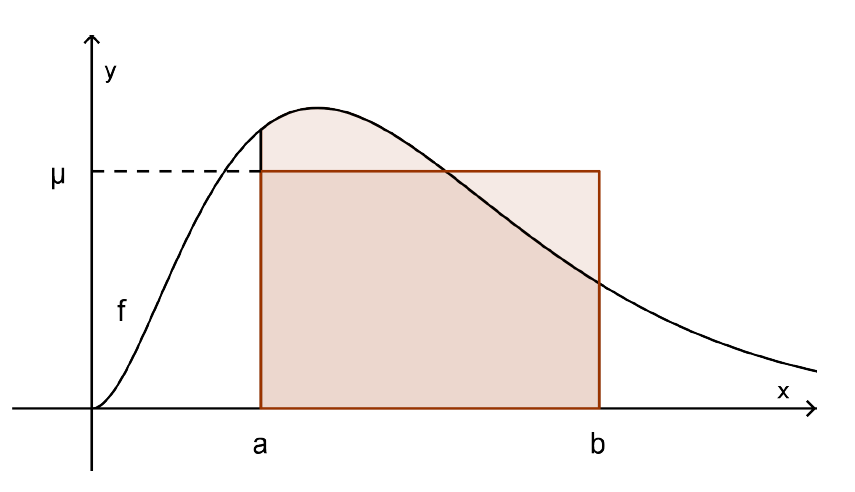
\includegraphics[width=0.4\textwidth]{images/Mittelwert_Grafik.png}
    \end{center}
  Definition des Mittelwert \(\mu\) der Funktion \(f(x)\) auf \([a,b]\): Höhe des Rechtecks, das
  \itemize
    \item eine Grundlinie der Länge \(b-a\) hat
    \item der Flächeninhalt des Rechteks der Fläche unter der Kurve \(f(x)\) im Intervall \([a,b]\) entspricht
	\[\mu = \frac{1}{b-a}\int_a^b{f(x)\mathrm{d}x} \]
\end{theorem}
\begin{formula}{Rotationsvolumen}\\
    \[V = \pi \int_a^b{(f(x))^2\mathrm{d}x} \]
\end{formula}
\begin{formula}{Bogenlänge}\\
    \[L=\int_a^b{\sqrt{1+(f'(x))^2}\mathrm{d}x} \]
\end{formula}
\begin{formula}{Mantelfläche}
    \[M=2\pi \int_a^b{f(x)\cdot \sqrt{1+(f'(x))^2}\mathrm{d}x} \]	
\end{formula}
\begin{theorem}{Schwerpunkt ebener Fläche}\\
  \begin{center}
  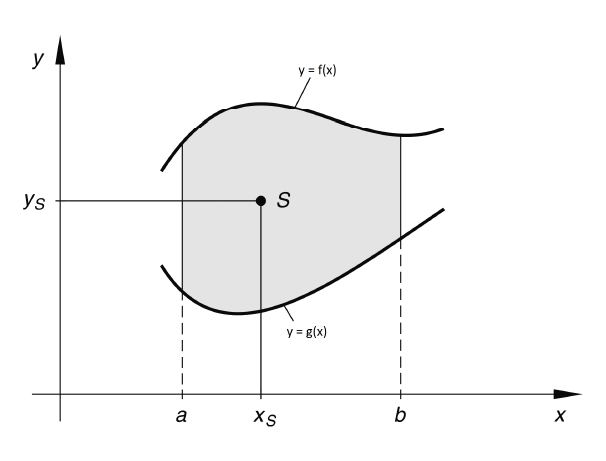
\includegraphics[width=0.4\textwidth]{images/Schwerpunkt_Beispiel.png}
  \end{center}
Schwerpunkt \(S=(x_s;y_s)\) einer ebenen Fläche mit Flächeninhalt A, eingegrenzt von Kurven \(y=f(x)\) und \(y=g(x)\)
sowie den Geraden \(x=a\) und \(x=b\):
\[xs = \frac{1}{A}\int_a^b{x\cdot(f(x)-g(x))\mathrm{d}x} \]
\[ys = \frac{1}{2A}\int_a^b{x\cdot(f(x)^2-g(x)^2)\mathrm{d}x} \]
Berechnen von \(A\) ebenfalls durch ein Integral:
\[A=\int_a^b{f(x)-g(x)\mathrm{d}x} \]
\end{theorem}
\begin{theorem}{Schwerpunkt Rotationskörper}\\
    Die x-Koordinate des Schwerpunkts \(S=(x_s;0;0) \) eines Rotationskörpers mit Volumen \(V\), geformt durch Rotation
    von \(y=f(x)\) zwischen \([a,b]\) um x-Achse mit \(a<b\) und \(f(x) \ge 0 \) für alle \(a \le x \le b \):
    \[x_s = \frac{\pi}{V}\int_a^b{x\cdot f(x)^2\mathrm{d}x} \]
\end{theorem}

\begin{KR}{Integrieren von Flächen}
    Nullstellen bestimmen: $=>$ Fläche oberhalb $\mathrm{x}$ Achse, + Fläche evtl unterhalb x Achse...
    \end{KR}
